\chapterimage{Week2AS.jpg}
\chapter{Activated Sludge}
		
		\section{Microbiology}\index{Microbiology}		
\begin{itemize}
\item The essence of the activated sludge system is to develop and and maintain a diverse population of microorganisms (activated sludge) that treats wastewater and which can be managed.
\item The activated sludge should be such that it \hl{not only effectively remove the BOD}, but also \hl{produces a floc that settles and compacts well} in the secondary clarifier thereby producing a secondary effluent with a low BOD content.
\item The floc produced has a porous structure and is essentially an aggregate of bacteria and extracelular material including organic polymers - polysaccharides and other substances secreted by the microorganisms, and remnants of dead microorganisms.  
\item Typically, the trophic organisms such as the protozoas and rotifers which feed on the bacteria and other particulates are generally present on the outer surface of the flocs.
\item A good quality activated sludge is brown in color with some froth and a slight musty odor.  
\item The settleability of the sludge is measured as SVI which is the volume of settled sludge in milliliters occupied by 1 gram of dry sludge solids after 30 minutes of settling in a 1,000 mL graduated cylinder or a settleometer.  
\item SVI of a good settling sludge is typically between 50 - 150 ml/g.\\ 
\item MCRT is the key factor which establishes the organism mix in the activated sludge.  
\item As MCRT increases, the size and complexity of the organisms increases.  
\item The types of organisms predominating in the Mixed Liquor give an indication as to the age of the sludge.
\begin{enumerate}[1.]  
\item At low MCRT of about less than 4 days the simpler protozoas - amoebae and flagellates dominate. 
\item With an increase in MCRT more complex organisms such as the free swimming ciliates and stalked ciliates appear. 
\item At even higher MCRT, metazoans such as the rotifers and nematodes may be found
\end{enumerate}

%Following is a chart showing the relative predominance of the trophic microorganisms with respect to the MCRT and its counterpart F:M.

%\begin{center}
%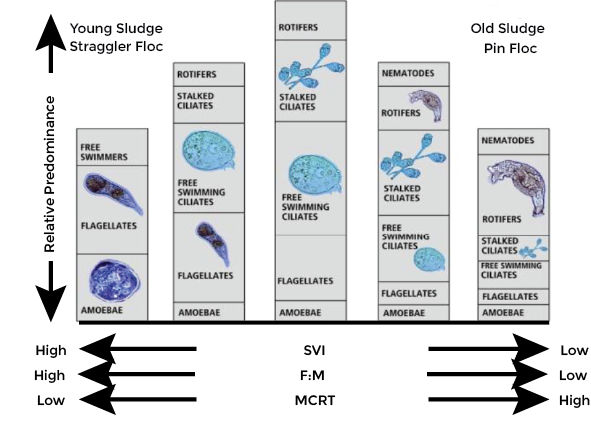
\includegraphics[scale=0.85]{ASRelativePredominance1}
%\end{center}

The most common activated sludge quality issues include:
\begin{enumerate}[1.]
\item Straggler floc:  This condition shows small, light, and fluffy floc particles with poor settling characteristics. It occurs due to young sludge or low MCRT/MLSS levels and may be related to an inadequate microorganism population or an excessive BOD load (high F:M) which causes a log growth situation. The cells become dispersed rather than flocculated, settleability is poor, and the effluent becomes turbid. In this condition oxygen is used up quickly due to the high metabolism rate, and sludge production is high. One tell-tale sign of this condition is the production of huge amounts of a billowing white foam.

\item Pin floc (Dispersed Growth):  Here flocs - pin floc is seen in the effluent. These are larger dimension spherical particles.  The sludge settles well in the settleability test but the supernatant is cloudy. This floc consist mostly of floc-forming bacteria without a filament backbone.  This condition occurs at starvation condition when all of the influent BOD has been used up (low F:M) and the old sludge age organisms are now in endogenous respiration.  Pin floc 

\item Rising sludge: Under this condition, sludge settles well, compacts on the bottom of the clarifier, then starts to rise in clumps and patches to the surface.  Rising sludge is typically evidenced as brown in color.  Rising sludge occurs due to either denitrification or sludge septicity due to an excessive detention time in the clarifier.  

\item Bulking and Foaming:  Typical bacteria present in activated sludge include spherical, rod shaped and filamentous.  The presence of filamentous bacteria in activated sludge provide the important structural element for the bacterial floc.  Bulking is indicated by SVI > 150 ml/g. However, certain condition cause an excessive growth of filaments which interferes with the settling (bulking) and cause foaming during aeration.   Identifying which filaments are dominating in the system through a microscopic evaluation will help the operator to understand the condition in the treatment system so that corrective changes can be made.\\

\begin{center}
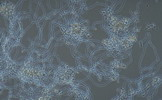
\includegraphics[scale=1]{Filaments}\\
Filaments proliferation
\end{center}

\end{enumerate}
\begin{enumerate}[a.]

\item Bulking:  Activated sludge bulking is marked by poor compaction – high SVI\textsubscript{30} and poor solids-liquid separation evidenced by high effluent TSS.  To resolve bulking issue, it is important to find its cause and take remedial actions.  This is accomplished through a microscopic examination to identify the type of the filament to provide a clue on the cause.  Short term remedy to bulking includes Chlorinating – 2-3 mg/l per 1000 lbs MLVSS or use of polymers.
\pagebreak

\begin{tabular}{ | m {4 cm} | m {2.5 cm}| m {10 cm}| } 
 \hline
\begin{center}\textbf{Filament Type}  \end{center} & \begin{center} \textbf{Cause} \end{center} & \begin{center} \textbf{Remedy} \end{center}\\
 \hline
\small S.natans, Type 1701 and H.hydrossis & \small Low D.O. ( For the applied organic loading )& \small Low aeration basin DO concentration for the applied F/M leads to filamentous bulking by several filaments.  Typically a minimum DO of 2 mg/l is required for F:M upto 0.5. The condition may also be remedies by raising the MLSS concentration (decreasing the F/M)\\ 
 \hline
\small M.parvicella, Nocardia species, Type 0041, Type 0675, Type 1851 and Type 0803 & \small Low Organic Loading Rate ( Low F:M )& \small Increase the F:M by reducing the MLSS concentration. When reduction in the MLSS concentration may not be feasible due to impact on nitrification, other suitable methods such as the use of a selector may be considered\\
 \hline
\small Thiothrix I and II, Beggiatoa species, N. limicola II, Type 021N, Type 0092, Type 0914, Type 0581, Type 0961 and Type 0411 & \small Septic Wastes / Sulfides ( High organic acids ) & \small Reduce septicity using pre-aeration and through use of chemicals which prevent septicity and reduce sulfides \\
 \hline
\small Thiothrix I and II and Type 021N (N defeciency)
N. limicola III (P defeciency)& \small Nutrient Deficiency ( N and / or P ) ( Industrial Wastes Only ) & \\
 \hline
Nocardia species, M.parvicella and Type 1863 & High Grease / Oil & \\
 \hline
\small Fungi & \small Low pH ( Below pH 6.0 ) / Oil  & \small The aeration basin pH should be maintained in the range 6.5 to 8.5. Low pH, <6.5, may cause the growth of fungi and fungal bulking. The aeration basin pH can be adjusted using caustic, lime or magnesium hydroxide.\\
 \hline
\end{tabular}
\pagebreak

\item Foaming:  Activated sludge foaming is caused mostly by two filaments: Nocardia spp. and Microthrix parvicella (there are other non-filament causes of foaming - including excessive presence of surfactants. Both of these filaments have three causes in combination: (1) high grease and oil; (2) longer sludge age; and (3) low oxygen conditions or septicity.  Foaming if left uncontrolled could potentially pose a permit compliance issue if the foam spills into the effluent.  Additionally, Nocardia from the secondary sludge could cause digester foaming.
\end{enumerate}